
The stated long term plan for nuclear deployment in France targets a technology 
transition to \glspl{SFR}\cite{cne2_reports_2015}. However, the current inventory of French \gls{UNF} 
is insufficient to fuel that transition without building new \glspl{LWR}.

If instead, France accepted 
\gls{UNF} from other \gls{EU} nations and used it to produce \gls{MOX} for new \glspl{SFR},
the \gls{MOX} created will fuel a French transition to an \gls{SFR} fleet
and allow France to avoid building additional \glspl{LWR}.

I used \Cyclus to simulate
 \gls{EU} spent nuclear material inventory accumulation and to model the 
 proposed French 
 technology transition from \glspl{LWR} to
 \glspl{SFR}. I calculated the used fuel
inventory in \gls{EU} member states and propose a potential collaborative
strategy of used fuel management.

Past research focuses solely on France and typically assumes that additional \glspl{LWR},
namely \glspl{EPR}, supply the \gls{UNF} required to produce \gls{MOX} 
\cite{carre_overview_2009, martin_symbiotic_2017, freynet_multiobjective_2016, merino_rodriguez_analysis_2014}.
The strategies in these works estimate full \gls{SFR} transition in 2100.
Other recent work in the literature investigates partitioning and transmutation
in a European context, with \glspl{ADS} and Gen-IV reactors \cite{fazio_study_2013,
alvarez-velarde_analysis_2008},
to reduce radiotoxicity for disposal.
However, little recent work considers synergistic international spent fuel arrangements.
This work finds that a collaborative strategy can reduce the
need to construct additional \glspl{LWR} in France, if 
the \glspl{SFR} are as commercially competitive as recent work
suggests they may be \cite{zhao_improving_2009}.

This chapter details that French \gls{NFC} transition
scenario from an \gls{LWR} fleet to a fully \gls{SFR} fleet.
I show that if France accepts \gls{UNF} from other \gls{EU} nations,
it will reach its desired \gls{SFR} end-goal more rapidly.


\section{\gls{EU} deployment schedule}

The historic \gls{EU} deployment schedule and operation history 
are generated using the \texttt{from\_pris.py}
module (described in section \ref{sec:writeinput}).

Projections of future reactor deployment in this simulation are based on
assessment of analyses from references, for instance \gls{PRIS}, for reactors planned
for construction \cite{iaea_nuclear_2017}, the World Nuclear Association
\cite{world_nuclear_association_nuclear_2017}, and literature concerning the future of
nuclear power in a global \cite{joskow_future_2012} and European context
\cite{hatch_politics_2015}.  Existing projections extend to 2050.

Table \ref{tab:eu_deployment} lists the reactors that are currently  planned or
under construction in the \gls{EU}. In the simulation, all  planned constructions are completed 
without delay or failure and reach a lifetime of 60 years.  

\pagebreak
\begin{table}[h]
    \centering
    \caption {Power reactors under construction and planned. Replicated from \cite{world_nuclear_association_nuclear_2017}.}
    \label{tab:eu_deployment}
    \begin{tabular}{ccccr}
        \hline
        \textbf{Exp. Operational }&\textbf{Country} &\textbf{Reactor} & \textbf{Type} & \textbf{Gross MWe}\\
        \hline
        2018 & Slovakia  & Mochovce 3 & PWR & 440\\
        2018 & Slovakia & Mochovce 4 & PWR & 440 \\
        2018 & France & Flamanville 3 & PWR & 1600 \\
        2018 & Finland & Olkilouto 3 & PWR & 1720 \\
        2019 & Romania & Cernavoda 3 & PHWR & 720 \\
        2020 & Romania & Cernavoda 4 & PHWR & 720 \\
        2024 & Finland & Hanhikivi & VVER1200 & 1200 \\
        2024 & Hungary & Paks 5 & VVER1200 & 1200 \\
        2025 & Hungary & Paks 6 & VVER1200 & 1200 \\
        2025 & Bulgaria & Kozloduy 7 & \footnotemark AP1000 & 950 \\
        2026 & UK & Hinkley Point C1 & EPR & 1670 \\
        2027 & UK & Hinkley Point C2 & EPR & 1670 \\
        2029 & Poland & Choczewo & N/A & 3000 \\
        2035 & Poland & N/A & N/A & 3000 \\
        2035 & Czech Rep & Dukovany 5 & N/A & 1200 \\
        2035 & Czech Rep & Temelin 3 & AP1000 & 1200 \\
        2040 & Czech Rep & Temelin 4 & AP1000 & 1200 \\
        \hline
    \end{tabular}
\end{table}

    \footnotetext{The fate of many planned reactors is uncertain. The proposed reactor types
              are also unclear. The ones marked `N/A' for type are assumed to the \glspl{PWR}
              in the simulation.}
\FloatBarrier

For each \gls{EU} nation, I categorized the growth trajectory from
``Aggressive Growth'' to ``Aggressive Shutdown''. ``Aggressive growth'' is
characterized by a rigorous expansion of nuclear power, while
``Aggressive Shutdown'' is characterized as a transition to rapidly
de-nuclearize the nation's electric grid. I categorized each nation's growth 
trajectory into five degrees depending on G, the growth trajectory metric:

 \[
 G = \left\{\begin{array}{ll}
 \text{Aggressive Growth}, & \text{for } G \geq 2\\
 \text{Modest Growth}, & \text{for } 1.2 \leq G < 2\\
 \text{Maintenance}, & \text{for } 0.8 \leq G < 1.2 \\
 \text{Modest Reduction}, & \text{for } 0.5 \leq G< 0.8\\
 \text{Aggressive Reduction}, & \text{for } G \leq 0.5
 \end{array}\right\} = \frac{C_{2040}}{C_{2017}}\\\\
 \]
 \[
  G = \text{Growth Trajectory  } [-] 
 \]
 \[
 C_{i} = \text{Nuclear Capacity in Year i  } [\gls{MWe}].
 \]

The growth trajectory and specific plan of each nation in the \gls{EU} 
is listed in Table \ref{tab:eu_growth}.  

\begin{table}[h]
    \centering
    \caption{Projected nuclear power strategies of \gls{EU} nations \cite{world_nuclear_association_nuclear_2017}}
        \begin{tabular}{lll}
            \hline 
                    \textbf{Nation} & \textbf{Growth Trajectory} & \textbf{Specific Plan }\\
                    \hline
                    UK & Aggressive Growth & {\small  13 units (17,900 \gls{MWe}) by 2030.}\\
                    Poland & Aggressive Growth &  {\small Additional 6,000 \gls{MWe} by 2035.}\\
                    Hungary & Aggressive Growth &  {\small Additional 2,400 \gls{MWe} by 2025.} \\ 
                    Finland & Modest Growth &  {\small Additional 2,920 \gls{MWe} by 2024.}\\
                    Slovakia & Modest Growth & {\small Additional 942 \gls{MWe} by 2025.}\\
                    Bulgaria & Modest Growth &  {\small Additional 1,000 \gls{MWe} by 2035.} \\
                    Romania & Modest Growth &  {\small Additional 1,440 \gls{MWe} by 2020.} \\
                    Czech Rep. & Modest Growth & {\small  Additional 2,400 \gls{MWe} by 2035.}\\
                    France & Modest Reduction & {\small No expansion or early shutdown.}\\
                    Slovenia & Modest Reduction & {\small No expansion or early shutdown.}\\
                    Netherlands & Modest Reduction & {\small No expansion or early shutdown.}\\
                    Lithuania & Modest Reduction & {\small No expansion or early shutdown.}\\
                    Spain & Modest Reduction &  {\small No expansion or early shutdown.} \\
                    Italy & Modest Reduction & {\small No expansion or early shutdown. }\\
                    Belgium & Aggressive Reduction & All shut down 2025.\\
                    Sweden & Aggressive Reduction & All shut down 2050.\\
                    Germany & Aggressive Reduction & All shut down by 2022.\\
                    \hline
                    
        \end{tabular}
  \label{tab:eu_growth}
\end{table}
\FloatBarrier


Using this categorization to drive facility deployment, \Cyclus captures 
regional differences in reactor power capacity and \gls{UNF} production as a 
function of time. Accordingly, figure \ref{fig:eu_pow} shows the resulting simulated 
installed capacity in \gls{EU} nations.  Sudden capacity reductions seen in the 
2040s result from end-of-license reactor retirements and nuclear phaseout plans 
in nations such as Germany and Belgium.  

\begin{figure}[htbp!]
    \begin{center}
        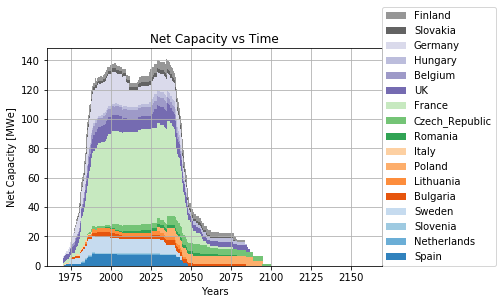
\includegraphics[scale=0.7]{./images/eu_future/power_plot.png}
    \end{center}
    \caption{Installed nuclear capacity in the EU is distinguished by \texttt{Region}s in \Cyclus.
             The large drops near 2025 is due to the nuclear phase-out plans in Germany and Belgium.}
    \label{fig:eu_pow}
\end{figure}



\section{French \gls{SFR} deployment schedule}

Figure \ref{fig:sfr_num}
shows
the French transition to \glspl{SFR} modeled in this simulation.
Historically aggressive growth of nuclear in the 1980s leads to a substantial 
shutdown of nuclear in the 2040s, which, in the simulation, are replaced by new 
\glspl{SFR}. The net capacity is kept constant at 64.7 GWe.

\begin{figure}[htbp!]
        \begin{center}
                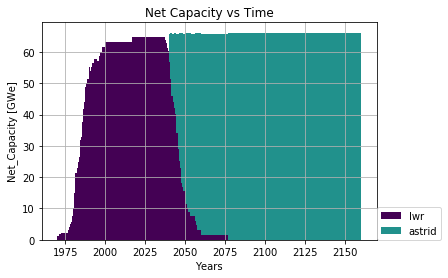
\includegraphics[scale=0.7]{./images/french-transition/power_plot.png}
        \end{center}
        \caption{The potential French transition from \glspl{LWR} to 
                \glspl{SFR} when assisted by \gls{UNF} from other \gls{EU} 
        nations.}
        \label{fig:sfr_num}
\end{figure}

Figure \ref{fig:french_dep} shows the deployment strategy required to support the transition in 
figure \ref{fig:sfr_num}. France must build 1.78 \glspl{ASTRID} per year, on average, to 
make up for the end-of-license decommissioning of power plants built in the 1980s and 1990s.
The second period of aggressive building occurs when the first generation of \glspl{SFR} decommission after 80 years.
Starting in 2040, France deploys 600-\gls{MWe} \glspl{SFR} to make up for 
decommissioned French \gls{LWR} capacity. This results in an installed 
\gls{SFR} 
capacity of 64,700 \gls{MWe} by 2078 when the final \gls{LWR} is 
decommissioned. 



\begin{figure}[htbp!]
    \begin{center}
        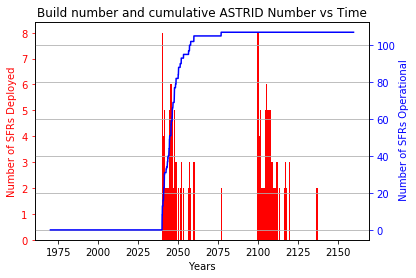
\includegraphics[scale=0.7]{./images/french-transition/sfr_deploy.png}
    \end{center}
    \caption{The simulated deployment of \glspl{SFR} in France is characterized by a period of
    aggressive building.}
    \label{fig:french_dep}
\end{figure}


Finally, figure \ref{fig:tot_dep} shows the total deployment scheme I simulated.  
The French transition to \glspl{SFR} couples with the historical and projected 
operation of \gls{EU} reactors.  The steep transition from 2040 to 2060 
reflects the scheduled decommissioning of reactors built in the 1975-2000 era 
of aggressive nuclear growth in France.

\begin{figure}[htbp!]
    \begin{center}
        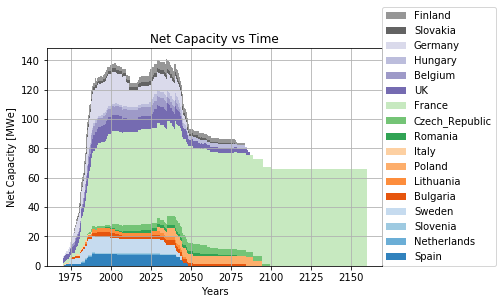
\includegraphics[scale=0.7]{./images/eu_future/onesim.png}
    \end{center}
    \caption{The total simulated deployment scheme relies on \gls{UNF} 
    collaboration among nations.} 
    \label{fig:tot_dep}
\end{figure}

These figures reflect that, for the given assumptions, bursts of construction
are necessary to maintain capacity.  In reality, a construction rate of five 
reactors every year is ambitious, but might have the advantage of
larger scale production of components and more modular assembly and construction if major components can mostly be built off site.

Alternatively, the 
deployment of new \glspl{SFR} can be spread out by staggering scheduled 
decommissioning of \glspl{LWR} through lifetime extensions. For example,
I increased the original lifetime of French \glspl{LWR} (60 years) randomly 
by sampling from a uniform distribution of lifetime extension
magnitudes between 0 and 25 years. 
This results in a more gradual transition and \gls{ASTRID} construction
burden, as shown in figure \ref{fig:sfr_num_norm} and \ref{fig:sfr_dep_norm}.
The effect of \gls{LWR} lifetime extension is discussed in Section \ref{sec:life}.

\begin{figure}[htbp!]
	\begin{center}
		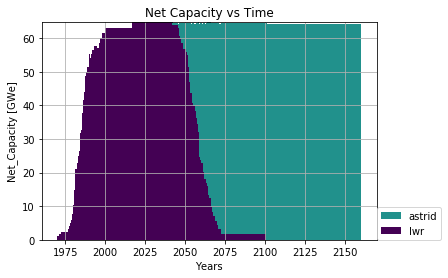
\includegraphics[scale=0.7]{./images/french-transition/unif_0_25.png}
	\end{center}
	\caption{The transition to \glspl{ASTRID}
		becomes more gradual if the
		French \gls{LWR} lifetime extensions are sampled from a 
		uniform distribution $\in [0, 25]$ years.}
	\label{fig:sfr_num_norm}
\end{figure}

\begin{figure}[htbp!]
	\begin{center}
		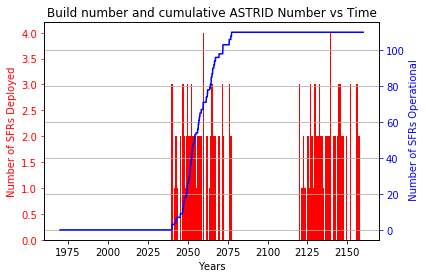
\includegraphics[scale=0.7]{./images/french-transition/unif_0_25_dep.png}
	\end{center}
	\caption{The acute construction burden lessens if the
		French \glspl{LWR} lifetime extensions are sampled from a 
		uniform distribution $\in [0, 25]$ years.}
	\label{fig:sfr_dep_norm}
\end{figure}

\FloatBarrier

This analysis establishes a multi-national material flow and demonstrates that, if such an aggressive deployment scheme took place, the \glspl{SFR} would have enough fuel.

\section{Material flow}

The fuel cycle is represented by a series of facility agents whose material 
flows are illustrated in figure \ref{diag:fc}, along with
the \Cyclus archetypes that were used to model each facility.
In this diagram, \gls{MOX} Reactors include both French \glspl{PWR} and 
\glspl{SFR}.

% Define block styles
\tikzstyle{decision} = [diamond, draw, fill=blue!20, 
text width=4.5em, text badly centered, node distance=3cm, inner sep=0pt]
\tikzstyle{block} = [rectangle, draw, fill=blue!20, 
text width=5em, text centered, rounded corners, minimum height=4em]
\tikzstyle{line} = [draw, -latex']
\tikzstyle{cloud} = [draw, ellipse,fill=red!20, node distance=3cm,
minimum height=2em]


\begin{figure}
	\centering
	\scalebox{0.6}{
		\begin{tikzpicture}[align=center, node distance = 3cm and 3cm, auto]
		% Place nodes
		\node [block] (sr) {Mine (\texttt{SOURCE})};
		\node [cloud, below of=sr] (nu) {Nat U};
		\node [block, below of=nu] (enr) {\small Enrichment ({\scriptsize \texttt{ENRICHMENT}})};
		\node [cloud, below of=enr] (uox) {\acrshort{UOX}};
		\node [block, below of=uox] (lwr) {\gls{LWR} (\texttt{REACTOR})};
		\node [cloud, right of=lwr] (snf) {\gls{UNF}};
		\node [block, right of=snf] (pool) {Pool (\texttt{Storage})};
		\node [cloud, left of=lwr] (tl2) {Dep U};
		\node [cloud, right of=enr] (tl) {Dep U};
		\node [block, right of=tl] (sk) {Repository (\texttt{SINK})};
		\node [cloud, below of=sk] (cunf) {Cooled \gls{UNF}};
		\node [cloud, below of=pool] (cunf2) {Cooled \gls{UNF}};
		\node [block, below of=snf] (rep) {{\footnotesize Reprocessing ({\scriptsize \texttt{SEPARATIONS}})}};
		\node [cloud, below of=rep] (u) {Sep. U} ;
		\node [cloud, left of=rep] (pu) {Sep. Pu};
		\node [block, left of=pu] (mix) {Fabrication (\texttt{MIXER})};
		\node [cloud, below of=mix] (mox) {\gls{MOX}};
		\node [block, below of=mox] (mxr) {\gls{MOX} Reactors 
			(\texttt{REACTOR})};
		\node [cloud, right of= mxr] (snmox) {Spent \gls{MOX}};
		
		\draw[->, thick] (sr) -- (nu);
		\draw[->, thick] (nu) -- (enr);
		\draw[->, thick] (enr) -- (tl);
		\draw[->, thick] (enr) -- (tl2);
		\draw[->, thick] (tl) -- (sk);
		\draw[->, thick] (tl2) -- (mix);
		\draw[->, thick] (enr) -- (uox);
		\draw[->, thick] (uox) -- (lwr);
		\draw[->, thick] (lwr) -- (snf);
		
		\draw[->, thick] (lwr) -- (snf);
		\draw[->, thick] (snf) -- (pool);
		\draw[->, thick] (pool) -- (cunf);
		\draw[->, thick] (pool) -- (cunf2);
		\draw[->, thick] (cunf) -- (sk);
		\draw[->, thick] (cunf2) -- (rep);
		
		\draw[->, thick] (rep) -- (u);
		\draw[->, thick] (rep) -- (pu);
		\draw[->, thick] (pu) -- (mix);
		\draw[->, thick] (mix) -- (mox);
		\draw[->, thick] (mox) -- (mxr);
		\draw[->, thick] (mxr) -- (snmox);
		\draw[->, thick] (snmox) -- (rep);
		
		\end{tikzpicture}
		
	}
	\caption{Fuel cycle facilities (blue boxes) represented by 
		\Cyclus archetypes (in parentheses) pass materials (red 
		ovals) around the simulation.} 
	\label{diag:fc}
\end{figure}

A mine facility provides natural uranium, which is enriched by an enrichment
facility to produce \gls{UOX}. Enrichment wastes (tails) are disposed of to a 
sink facility representing ultimate disposal. The enriched \gls{UOX} fuels
the \glspl{LWR} which in turn produce spent \gls{UOX}. The used fuel
is sent to a wet storage facility for a minimum of 72 months. \cite{carre_overview_2009}.

The cooled fuel is then reprocessed to separate plutonium and uranium,
or sent to the repository.
The plutonium mixed with depleted uranium (tails) makes \gls{MOX} (Both for
French \glspl{LWR} and \glspl{ASTRID}).
Reprocessed uranium is unused and stockpiled. Uranium is reprocessed
in order to separate the raffinate (minor actinides and fission products)
from usable material. Though neglected in this work, reprocessed
uranium may substitute depleted uranium for \gls{MOX} production. In the
simulations, sufficient depleted uranium existed that the complication of
preparing reprocessed uranium for incorporation into reactor fuel
was not included. However, further in the future when the depleted
uranium inventory drains, reprocessed uranium (or, natural uranium) will need to be utilized. 

\FloatBarrier

\section{Scenario specification}

The scenario specifications defining the simulations presented in this work 
are listed in table \ref{tab:gen}.
The reprocessing and \gls{MOX} fabrication capacity in France
prior to 2020 is modeled after the 
French La Hague and MELOX sites \cite{schneider_spent_2008, hugelmann_melox_1999}.


\begin{table}[h]
    \centering
    \caption{Simulation Specifications}
    \begin{tabularx}{\linewidth}{bRR}
        \hline
        \textbf{Specification} &\textbf{Value} & \textbf{Units}\\
        \hline
        Simulation Starts & 1970 & year\\
        Simulation Ends & 2160 & year\\
        Production of \gls{ASTRID} fuel begins & 2020 & year\\
        \glspl{SFR} become available & 2040 & year\\
        Reprocessed uranium usage &  Not used & -\\
        Minimum \gls{LWR} \gls{UNF} cooling time  & 72  & months \\
        Minimum \gls{ASTRID} \gls{UNF} cooling time  & 36  & months\\
        Separation efficiency of U and Pu & 99.8 & \% \\
        Reprocessing streams & Pu and U & - \\
        Reprocessing capacity before 2020 & 91.6 \cite{schneider_spent_2008} & \gls{MTHM}/month  \\
        Reprocessing capacity after 2020 & 183.2 & \gls{MTHM}/month\\
        \gls{LWR} \gls{MOX} fabrication throughput & 16.25 \cite{hugelmann_melox_1999} & \gls{MTHM}/month\\
        \gls{ASTRID} \gls{MOX} fabrication throughput & No limit ($\infty$) & \gls{MTHM}/month \\
        \gls{LWR} \gls{MOX} recycling  &  Not reprocessed & - \\
        \gls{ASTRID} \gls{MOX} recycling & $\infty$-pass & - \\
        \hline
    \end{tabularx}
    \label{tab:gen}
\end{table}



\pagebreak

\section{Reactor specifications}
Three major reactors are used in the simulation, \gls{PWR}, \gls{BWR}, and ASTRID-type \gls{SFR} reactors.
The \gls{PWR} and \gls{BWR} specifications are determined using the linear core size model,
as explained in section \ref{sec:writeinput}. The ASTRID-type \gls{SFR} specification
is obtained from Varaine et al \cite{varaine_pre-conceptual_2012}.
The \gls{ASTRID} design's target lifetime is 60 years \cite{gauche_generation_2012}.

\begin{table}[h]
    \centering
    \caption{Baseline \gls{LWR} and \gls{ASTRID} simulation specifications.}
    \begin{tabular}{lrrr}
        \hline
        \textbf{Specification} & \textbf{\gls{PWR} \cite{sutharshan_ap1000tm_2011}} & \textbf{\gls{BWR} \cite{hinds_next-generation_2006}} & \textbf{\gls{SFR}} \cite{varaine_pre-conceptual_2012}\\
        \hline
                Lifetime \tablefootnote{The simulated reactor lifetime reaches the licensed lifetime unless 
        the reactor is shut down prematurely.} [y]  & 60 & 60 & 60 \\
                Cycle Time [mos.]& 18 & 18 & 12\\ 
                Refueling Outage [mos.]& 2 & 2  & 2\\
                Rated Power [\gls{MWe}] & 1110 & 1000 & 600\\
                Assembly mass [kg] & 446 & 180 & -- \\
                Batch mass [kg] & -- & -- & 5,568\\
                Discharge Burnup [GWd/tHM] & 51 & 51 & 105 \\
                Assemblies per core \tablefootnote{Number of assemblies and corresponding \gls{LWR} core 
        masses are reported for a 1100-\gls{MWe} core. Reactors with different core  
        powers are modeled with a linear mass assumption.} & 157  & 764 & -- \\

                Batches per core & 3 & 3 & 4\\
        Initial Fissile Loading [t] & 4.3  $^{235}$U & 5.8  $^{235}$U & 4.9 Pu \\
                Fuel & \gls{UOX} or \gls{MOX} & \gls{UOX} & \gls{MOX} \\
        \hline
    \end{tabular}
        
    \label{tab:reactor-specs}

    \end{table}



\section{Material definitions}
Depletion of the nuclear fuel is modeled with pre-calculated spent fuel recipes, such that a fresh 
and used fuel recipe are defined for each reactor type.
An ORIGEN reference calculation provides the composition of the used fuel (see table \ref{tab:eu_comp}).
ORIGEN calculates buildup, decay, and processing of radioactive materials
\cite{parks_overview_1992}. This recipe has also been used for repository performance modeling \cite{wilson_adoption_2009}.

\begin{table}[h]
    \centering
    \caption{Fresh fuel compositions in the simulation \cite{wilson_adoption_2009, varaine_pre-conceptual_2012}.}
%   \scalebox{0.86}{
        \begin{tabular}{lSSS}
            \hline
             & \multicolumn{3}{c}{ Composition [\%]} \\
            Recipe & \text{U235}  & \text{U238}  & Pu \\ 
            \hline
            Fresh \gls{UOX} Fuel & 4.29 & 95.71 & 0.0   \\ 
            Fresh \gls{LWR} \gls{MOX} Fuel & 0.2 & 90.7 & 9.1 \\ 
            Fresh \gls{ASTRID} Fuel & 0.3 & 77.7 & 22.0 \\
            \hline
        \end{tabular}
        
        \label{tab:eu_comp}
\end {table}


\section{Results}
This section describes the simulation results if France utilized
\gls{UNF} from other \gls{EU} nations to fuel the transition into a fully
\gls{ASTRID} fleet.

First, I confirm that France does not have enough
\gls{LWR} \gls{UNF} to transition into a fully \gls{SFR}
fleet. As shown in figure \ref{fig:only_france}, France
cannot meet the \gls{ASTRID} fuel demand without receiving
\gls{LWR} \gls{UNF} from other \gls{EU} nations. France
is able to fuel some of its \glspl{ASTRID} and breed more
plutonium, but cannot meet the fuel demand of 
all \glspl{ASTRID} with this aggressive deployment scheme.
\begin{figure}[htbp!]
	\begin{center}
		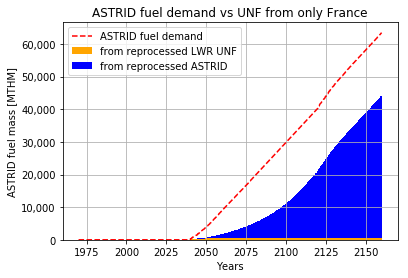
\includegraphics[scale=0.7]{./images/french-transition/france_only_compare.png}
	\end{center}
	\caption{\gls{ASTRID} fuel demand compared with fuel supply from only
		France in the simulation. The lack of initial \gls{ASTRID} fuel
		is caused by the lack of \gls{LWR} \gls{UNF} to reprocess. The
		initial shortage then causes a decrease in plutonium bred by
		\glspl{ASTRID}, thus a decrease in \gls{ASTRID} fuel supply.}
	\label{fig:only_france}
\end{figure}


\subsubsection{Nuclear fuel material inventory}
\Cref{tab:sim_result1}
lists predicted \gls{EU} material inventory in 2050.
While \gls{UNF} continues to accumulate after 2050, the
\gls{UNF} France receives before 2050 is most impactful for the
feasibility of the transition. Note that table \ref{tab:sim_result1} 
distinguishes the
stored \gls{UNF} from the \gls{UNF} reprocessed to create \gls{MOX}.


\begin{table}[h]
    \centering
        \caption{\gls{EU} nuclear material inventory in 2050.}
\begin{tabularx}{\textwidth}{XrX}
            \hline
                        \textbf{Category} & \textbf{Value} & Specifics \\
                                          & \textbf{[MTHM]} & \\ \hline
                        UOX Loaded  & 152,271 & UOX used in EU reactors 1970-2050\\ 
            MOX Loaded  & 6,463  & MOX used in French reactors 1970-2050\\
                        Available used UOX (EU)  & 85,111  & Used EU (minus France) 
                                UOX in storage for future ASTRID MOX 
                                production\\
                        Available used UOX (France) & 
                                12,582  & Used French UOX stored for 
                                future ASTRID MOX production. \\
                                Reprocessed UOX (France) & 51,511 & Used French UOX already reprocessed for the production of LWR MOX \\
            Tails  & 1,330,165  & (Tails generated) $-$ (Tails used for production of LWR MOX) \\ 
            Natural U Used  & 1,482,436  & \\ \hline
        \end{tabularx}
        
        \label{tab:sim_result1}
\end {table}
\FloatBarrier



Figures \ref{fig:eu_tail} and \ref{fig:eu_snf} show the 
accumulation of tails and used fuel over time in the \gls{EU}.
Tails accumulate as a by-product of uranium enrichment. 
Spent fuel is discharged from reactors every refueling period.
The entire core is discharged when the reactor decommissions.
A total of $1,330,165$ MTHM of tails and $85,111$ MTHM of
\gls{UNF} have accumulated by 2050.
Figure \ref{fig:eu_fuel} shows the amount of fuel used in the \gls{EU}. The 
tails mass accumulation rate is fairly steady, with peaks occurring when new 
reactors are deployed.
In figure \ref{fig:eu_snf}, the peaks are caused by reactor decommissioning which 
triggers all the batches in the final reactor core to be sent to the repository.


\begin{figure}[htbp!]
    \begin{center}
        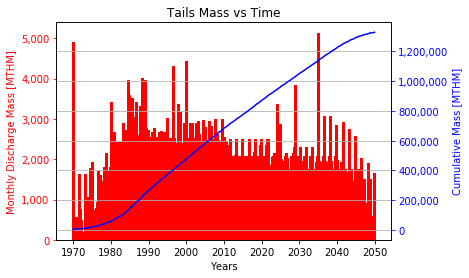
\includegraphics[scale=0.7]{./images/eu_future/tails.png}
    \end{center}
        \caption{Simulated accumulation of tails in the \gls{EU} is shown as a function of time.}
    \label{fig:eu_tail}
\end{figure}

\begin{figure}[htbp!]
    \begin{center}
        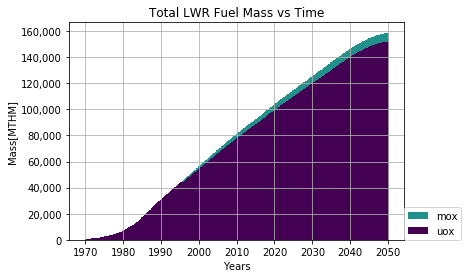
\includegraphics[scale=0.7]{./images/eu_future/total_fuel.png}
    \end{center}
\caption{Simulated total \gls{EU} fuel usage is shown as a function of time.}
    \label{fig:eu_fuel}
\end{figure}


\begin{figure}[htbp!]
    \begin{center}
            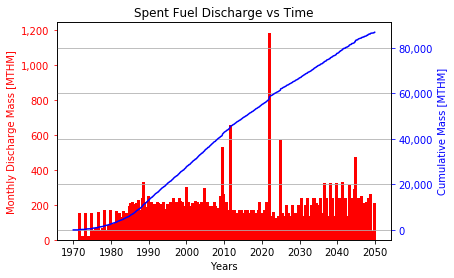
\includegraphics[scale=0.7]{./images/eu_future/snf_discharge.png}
    \end{center}
        \caption{Simulated \gls{EU} \gls{UNF} accumulation and discharge is 
shown as a function of time. The large peak near 2025 is due to the planned German
nuclear pahse-out, in which all German reactors will have been decommissioned by 2022.}
    \label{fig:eu_snf}
\end{figure}

\FloatBarrier
\subsubsection{French \gls{SFR} deployment}


Reprocessing the \gls{UNF} collected from all EU nations can provide 
approximately 913 tons of plutonium. Table \ref{tab:pu} lists the 
isotope, mass fraction, and quantity of plutonium that can be obtained from the 
2050 \gls{UNF} inventory.  With the \gls{SFR} breeding ratio above one, France 
can transition into a fully \gls{SFR} fleet without extra construction of 
\glspl{LWR}. 

\begin{table}[h]
    \centering
    \caption{Plutonium in the \gls{UNF} inventory.}
    \begin{tabular}{lSS}
        \hline
        \textbf{Isotope} & \textbf{Mass Fraction in Used Fuel [\%]} & \textbf{Quantity [t]} \\ \hline
        Pu238 & 0.011 & 9.76 \\ 
        Pu239 & 0.518 & 506.05 \\ 
        Pu240 & 0.232 & 226.64 \\ 
        Pu241 & 0.126 & 123.09 \\ 
        Pu242 & 0.048 & 47.57 \\ \hline
        \bfseries Total & 0.935 & 913.14 \\ \hline
    \end{tabular}
    
    \label{tab:pu}
\end{table}

From Varaine et al. \cite{varaine_pre-conceptual_2012}, a French
ASTRID-type 600\gls{MWe} \gls{SFR} consumes $1.125$ metric tons of
plutonium a year, with an initial plutonium loading of $4.9$ metric tons.

 Used \gls{MOX} from an ASTRID reactor is 23.95\% plutonium
in this simulation (see table \ref{tab:comp}), whereas fresh \gls{MOX} is 22\% plutonium.
The plutonium breeding ratio in this simulation is thus assumed to be
$\approx 1.08$.

Figure \ref{fig:fuel} shows MTHM of \gls{MOX} loaded in the \glspl{SFR} per month.  The plot 
has peaks during a period of aggressive deployment of \glspl{SFR} followed by 
an equilibrium at 83 \gls{MTHM}. The peaks reoccur with the deployment of the 
second generation of \glspl{SFR}.  The spikes are due to initial fuel demand 
corresponding to these new deployments.  The initial cores loaded into new 
\glspl{SFR} rely on the \gls{MOX} created from legacy \gls{UNF}. Once the 
deployed \glspl{SFR} create enough extra plutonium, the legacy \gls{UNF} is no 
longer used. Notably, this switch from a less preferred fuel origin to a more 
preferred fuel origin is handled automatically within \Cyclus via user-defined preferences 
within its dynamic resource exchange algorithm \cite{gidden_methodology_2016}.


\begin{figure}[htbp!]
    \begin{center}
        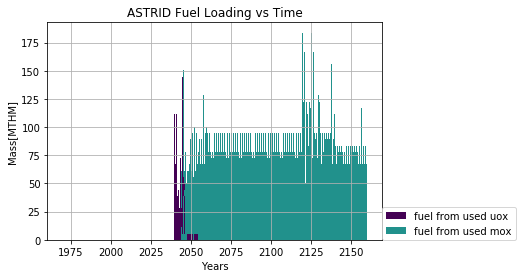
\includegraphics[scale=0.7]{./images/french-transition/where_fuel.png}
    \end{center}
    \caption{Fuel loaded into \glspl{SFR} was simulated in discrete 
        batches.}
    \label{fig:fuel}
\end{figure}

\Cref{fig:pu_no_cum} shows the separated plutonium discharge per month from the reprocessing plant.
The plutonium outflux does not precisely follow the fuel demand because \Cyclus agents have material
buffers that store commodity fuel for later usage. The reprocessed plutonium from legacy \gls{UNF} is
stored for the initial loading of \glspl{SFR}.  Plutonium separated from legacy \gls{UNF} meets
plutonium demans sufficiently to reduce the reprocessing demand for the first aggressive deployment
of \glspl{SFR}.  The plutonium from reprocessing legacy fuel is a flat rectangle because the reprocessing
throughput was set to 183.2 $\frac{\gls{MTHM}}{month}$ to avoid reprocessing all the legacy in one timestep.
This value is assuming that France doubles its current reprocessing capacity.
 

\begin{figure}[htbp!]
    \begin{center}
        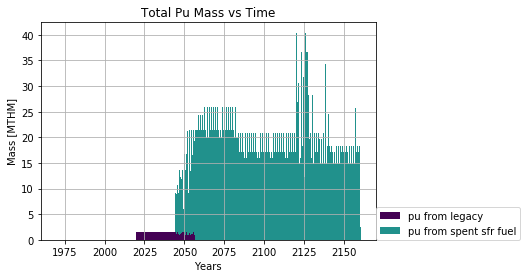
\includegraphics[scale=0.7]{./images/french-transition/pu.png}
    \end{center}
    \caption{The separated plutonium discharge from the reprocessing plant 
        in $\frac{\mbox{MTHM}}{\mbox{month}}$. The plutonium from \gls{LWR} \gls{UNF}
        is created after the demand is gone,  due to material buffers in \Cyclus.}
    \label{fig:pu_no_cum}
\end{figure}

Table \ref{tab:sfr_sim_result} lists French reprocessing and 
\gls{ASTRID} fuel fabrication metrics.

\begin{table}[h]
    \centering
    \caption {In the French transition to \glspl{SFR},
                  the total legacy \gls{UNF} reprocessed is the 
                                  amount of \gls{UNF} France needs 
                  for a transition into a fully \gls{SFR} fleet. 
                                  %The tails used is around ninth of the original tails inventory from the previous simulation.
                                  %KDH note: What does this mean?
                                  %thought there was only one simulation. . . 
                          }
        \begin{tabular}{llr}
            \hline
            \textbf{Category} & \textbf{Unit} & \textbf{Value}  \\ \hline
            Total \gls{ASTRID} MOX used & MTHM & 62,144  \\ 
            \textbf{Average UOX Reprocessing} & MTHM/month & \textbf{144.29} \\
            \textbf{Average Total Reprocessing} & MTHM/month & \textbf{61.3} \\
            \textbf{Average Fuel Fabrication} & MTHM/month & \textbf{36.9} \\
            Total \glspl{SFR} Deployed & & 214 \\ 
            Total Plutonium Reprocessed & MTHM & 13,671 \\ 
            Total \gls{ASTRID} fuel from UOX Waste & MTHM & 3,001  \\ 
            Total \gls{ASTRID} fuel from MOX Waste & MTHM  & 59,143 \\ 
            Total Tails used & MTHM & 48,472 \\ 
            \textbf{Total legacy UNF reprocessed} & MTHM & 55,553 \\ 
            Total Reprocessed Uranium Stockpile & MTHM & 194,186 \\ 
            Total Raffinate & MTHM & 12,123 \\ \hline
        \end{tabular}
        
        \label{tab:sfr_sim_result}
\end {table}

\FloatBarrier

These results demonstrate that despite the large amount of initial plutonium that has to be reprocessed
prior to \gls{ASTRID} deployment, the 20 years (2020-2040) of 
\gls{ASTRID} fuel preparation
allows a reasonable level of average
\gls{UOX} reprocessing capacity demand.

\section{Sensitivity analysis}

I explored the impact of two key variables, the lifetime of French
\glspl{LWR} and the breeding ratio of \gls{ASTRID} reactors. The range
of these parameters (table \ref{tab:sen_par}) sought to capture the full
span of their uncertainty.

Note that the breeding ratios of the \glspl{ASTRID} are artificially increased
by editing the output fuel composition in the \glspl{ASTRID}. I did not 
take into account the other reactor parameters (e.g. core size, initial
fuel composition, fuel residence time, etc.)
that must be changed to achieve these higher breeding ratios. More detailed analyses
of the reactor physics and their effect on this transition scenario are future work.

\begin{table}[h]
    \centering
    \caption{Both \gls{LWR} lifetime and \gls{ASTRID} breeding ratio impact 
    transitional reprocessing demand.}
    \begin{tabular}{lrr}
        \hline
        \textbf{Parameter} & \textbf{Default} & \textbf{Values} \\
        \hline
        Breeding Ratio of \glspl{ASTRID} & 1.08 & 1.11, 1.15, 1.18 \\ 
        Lifetime of French \glspl{LWR} [years] & 60  & 65, 70, 80 \\
        \hline
    \end{tabular}
    \label{tab:sen_par}
\end{table}

\subsection{Breeding Ratio}


Increase in the breeding ratio of \gls{ASTRID} reactors
decreases the total reprocessing demand, since less
\gls{UNF} must be reprocessed to extract the same amount of
plutonium. Additionally,
\glspl{ASTRID} become independent more quickly due to
higher breeding of plutonium.

Figure \ref{fig:br_fuel} shows the relationship between breeding ratio and fuel loading in \glspl{ASTRID}.
The \glspl{ASTRID} produce 
more plutonium, reducing the plutonium demand from 
reprocessed \gls{UOX}. However, since \gls{LWR} \gls{UNF} is not
the limiting factor for this transition scenario,
increasing the breeding ratio does not play a significant
role in the transition scenario, especially considering the technical difficulty
in achieving a high breeding ratio.

\begin{figure}[!ht]
	\centering
	\subfloat{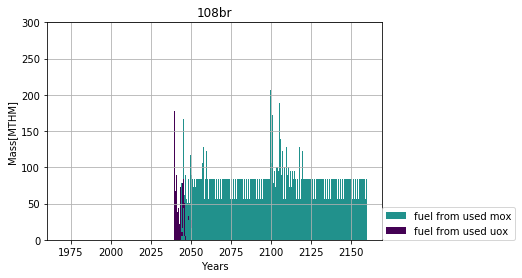
\includegraphics[width=.45\textwidth]{./images/sensitivity/108br.png}}\quad
	\subfloat{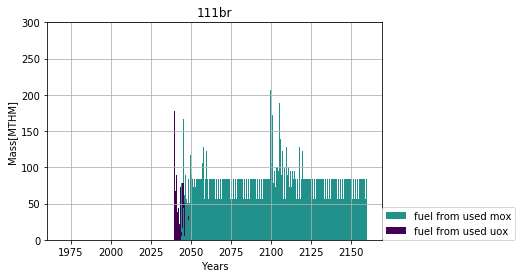
\includegraphics[width=.45\textwidth]{./images/sensitivity/111br.png}}\\
	\subfloat{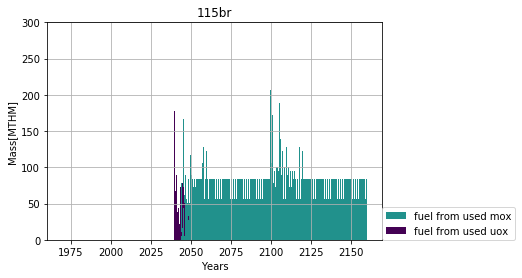
\includegraphics[width=.45\textwidth]{./images/sensitivity/115br.png}}\quad
	\subfloat{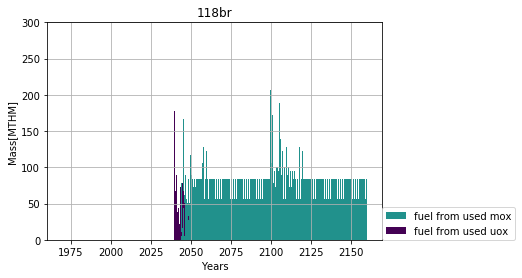
\includegraphics[width=.45\textwidth]{./images/sensitivity/118br.png}}
	\caption{\gls{ASTRID} fuel loading patters are altered by changes in \gls{ASTRID} 
		breeding ratio. Less \gls{ASTRID} fuel comes from reprocessed \gls{LWR} \gls{UNF}
		because \glspl{ASTRID} generate more plutonium.}
	\label{fig:br_fuel}
\end{figure}

The sensitivity analysis also shows, as demonstrated in figure \ref{fig:br_uox} that 
increasing the breeding ratio decreases the mass of \gls{LWR} \gls{UNF} 
required for the transition.

\begin{figure}[htbp!]
    \begin{center}
        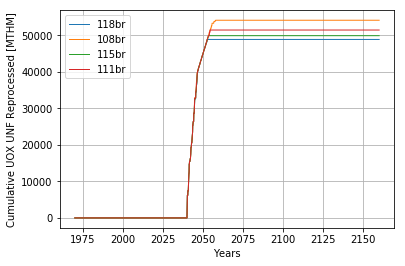
\includegraphics[scale=0.6]{./images/sensitivity/br_uox_unf_cum.png}
    \end{center}
    \caption{Sensitivity analysis demonstrates that increasing the breeding 
    ratio decreases the required \gls{UOX} \gls{UNF}. }
    \label{fig:br_uox}
\end{figure}

The differential impacts of varying the breeding ratios are
shown in table \ref{tab:br_diff}. The differences were calculated
using the following equation:

\[ \epsilon = \frac{(x - x_{base})}{x_{base}} * 100 \]

\begin{table}[h]
	\centering
        \caption{Breeding ratio impact on reprocessing requirements.}
	\begin{tabular}{lrrrr}
		\hline
                & \multicolumn{4}{c}{\% Difference} \\
		\textbf{Breeding Ratio $\longrightarrow$}& \textbf{1.08}& \textbf{1.11} & \textbf{1.15} & \textbf{1.18} \\
		\hline
		Total reprocessing demand & 0.0 & -5.3 & -7.8 & -10.3 \\ 
		\gls{LWR} \gls{UNF} reprocessed & 0.0  & -4.8 & -7.2 & -9.6 \\
		\hline
	\end{tabular}
	\label{tab:br_diff}
\end{table}


\subsection{Lifetime Extension of French \glspl{LWR}}\label{sec:life}
Extending the lifetime of French \glspl{LWR} lowers the average
monthly \gls{UOX} reprocessing demand, since the \gls{ASTRID} deployment becomes 
delayed (shown in figure \ref{fig:pow_diff}). The plutonium demand is delayed,
 allowing the reprocessing plant more time to prepare plutonium for \gls{ASTRID} reactors.

\begin{figure}[htbp!]
    \begin{center}
        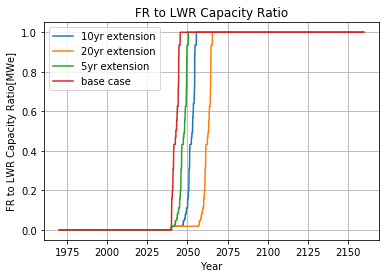
\includegraphics[scale=0.7]{./images/sensitivity/pow_ratio.png}
    \end{center}
    \caption{The ratio of \glspl{ASTRID} to \glspl{LWR} in France demarcates 
    the transition period.}
    \label{fig:pow_diff}
\end{figure}


Figure \ref{fig:ext_fuel} shows the change in \gls{ASTRID} fuel loading with
\gls{LWR} lifetime extension. The \gls{ASTRID} fuel loaded with plutonium
from \gls{LWR} \gls{UNF} conveys the corresponding \gls{LWR} \gls{UNF} reprocessing demand.
The change in \gls{ASTRID} deployment alters \gls{ASTRID} fuel loading patterns.
However, increasing the \gls{LWR} lifetimes
does not increase the \gls{LWR} \gls{UNF} demand significantly (less than 1\%
for the 20-year extension case),
because \glspl{ASTRID} become self-sustaining at similar times after the first
\gls{ASTRID} deployment.

\begin{figure}[!ht]
	\centering
	\subfloat{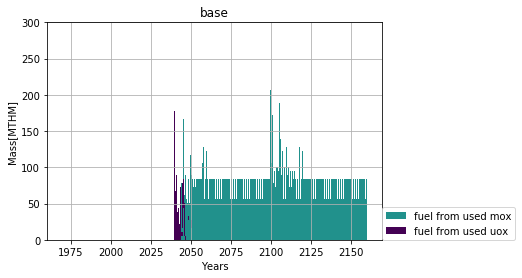
\includegraphics[width=.45\textwidth]{./images/sensitivity/base.png}}\quad
	\subfloat{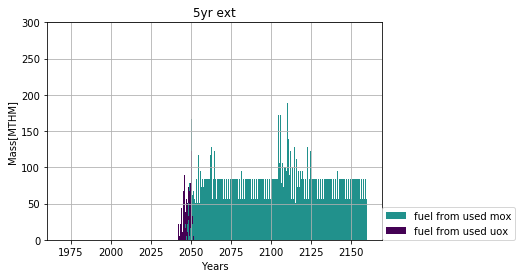
\includegraphics[width=.45\textwidth]{./images/sensitivity/5yr.png}}\\
	\subfloat{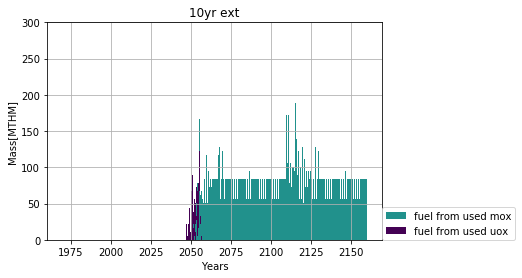
\includegraphics[width=.45\textwidth]{./images/sensitivity/10yr.png}}\quad
	\subfloat{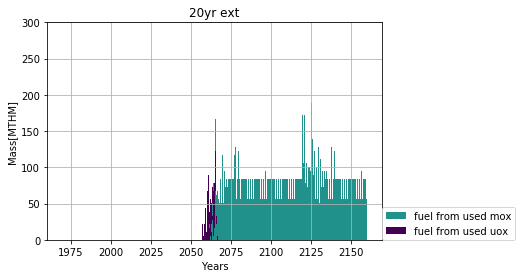
\includegraphics[width=.45\textwidth]{./images/sensitivity/20yr.png}}
	\caption{\gls{ASTRID} fuel loading patterns are altered by changes in \gls{ASTRID} deployment
			 caused by the lifetime extension of \glspl{LWR}.}
	\label{fig:ext_fuel}
\end{figure}

The quantitative effects of
\gls{LWR} lifetime extensions are shown in table \ref{tab:ext_met}.
The differences were calculated using the same equation used for the
breeding ratio study. 
Since \gls{LWR} lifetime extensions shorten the span of \gls{ASTRID} operations, less \gls{ASTRID} fuel is needed when \gls{LWR} lifetimes are extended.
Therefore, it is not fair to compare the mass of total \gls{UNF} reprocessed,
since less plutonium is extracted from \gls{UNF}. Instead, I compared the
average reprocessing values and the total amount of \gls{LWR} \gls{UNF} reprocessed.
There is not a significant difference (less than $1\%$ for the 20-year extension case)
in the amount of \gls{LWR}
\gls{UNF} reprocessed. The delay in \gls{ASTRID} deployment
spreads out the \gls{LWR} \gls{UNF} reprocessing demand,
thereby dramatically reducing ($39\%$ for the 20-year extension case)
the average monthly \gls{LWR} \gls{UNF} reprocessing demand.

\begin{table}[h]
	\centering
	\caption{\gls{LWR} lifetime extension impact on reprocessing requirements.}
	\begin{tabular}{lrrrr}
		\hline
		& \multicolumn{4}{c}{\% Difference} \\
		\textbf{\gls{LWR} lifetime extension $\longrightarrow$}& \textbf{0 years}& \textbf{5 years} & \textbf{10 years} & \textbf{20 years} \\
		\hline
		Total \gls{ASTRID} fuel produced & 0.0 & -3.9 & -8.0 & -16.3 \\
		\gls{LWR} \gls{UNF} reprocessed & 0.0  & -0.7 & -0.7 & -0.7 \\
		Average \gls{LWR} \gls{UNF} reprocessed & 0.0 & -16.0 & -25.7 & -39.8 \\
		Average \gls{UNF} reprocessed & 0.0 & -2.3 & -4.2 & -8.3 \\
		\hline
	\end{tabular}
	\label{tab:ext_met}
\end{table}


\FloatBarrier

\section{Conclusion}

France can transition into
a fully \gls{SFR} fleet with installed capacity of 64,700 \gls{MWe} without
building additional \glspl{LWR}
if France receives \gls{UNF} from other \gls{EU} nations.
Supporting the \gls{SFR} fleet requires an average 
reprocessing capacity of 61.3 \gls{MTHM} per month,
and an average fabrication capacity of 36.9 \gls{MTHM} per month.

The sensitivity study explored the effect of increased \gls{SFR} breeding
ratio and existing \gls{LWR} lifetime extension. Increasing the breeding
ratio reduced the amount of \gls{LWR} \gls{UNF} required to transition
up to $9.6\%$ and decreased the total reprocessing demand up to $10.3\%$.
Increasing the lifetime of existing \glspl{LWR} was not significant
in reducing the \gls{LWR} \gls{UNF} required to transition, but provided the benefit of
decreased average reprocessing demand due to delayed \gls{ASTRID} transition.

Since most \gls{EU} nations do not have an operating \gls{UNF}
repository or a management plan, they have a strong incentive
to send their \gls{UNF} to France. In particular, the nations
planning aggressive nuclear reduction will be able phase out nuclear
without constructing a permanent repository. France has an
incentive to take this fuel, since recycling used fuel from
other nations will allow France to meet their MOX demand
without new construction of \glspl{LWR}.

Table \ref{tab:which_send} lists \gls{EU} nations and their \gls{UNF} inventory
in 2050. I analyzed a strategy in which 
the nations reducing their nuclear fleet send their \gls{UNF} to France.
The sum of \gls{UNF} from Bulgaria, Poland, Czech Republic, Italy, Slovenia,
Belgium, Spain and Germany
provides enough \gls{UNF} for the simulated transition ($\approx 55,500$ MTHM). 
These nations are shown in bold in table \ref{tab:which_send}.
Sweden and Finland are not considered because they have established
national nuclear waste management plans.

If France receives \gls{LWR} \gls{UNF} from all \gls{EU} nations,
except Sweden and Finland,
it will have a surplus of $20,516$ MTHM of \gls{LWR} \gls{UNF}. This
inventory can be leveraged to increase nuclear power capacity as
the transition takes place. However, pragmatic limitations such
as new reactor construction, reprocessing throughput, and
political concerns remain.


\begin{table}[h]
    \centering
\begin{threeparttable}

    \caption {\gls{EU} nations and their respective \gls{UNF} inventory.} 
                \begin{tabular}{llr}
                    \hline 
                    \textbf{Nation} & \textbf{Growth Trajectory} & \small{\textbf{UNF in 2050 [MTHM] }}\\
                    \hline
                    \textbf{Poland} & \textbf{Aggressive Growth} & \textbf{1,807}\\
                    Hungary & Aggressive Growth & 3,119 \\ 
                    UK & Aggressive Growth & 13,157\\
                    Slovakia & Modest Growth & 2,744\\
                    \textbf{Bulgaria} & \textbf{Modest Growth} & \textbf{2,965} \\
                    \textbf{Czech Rep.} & \textbf{Modest Growth} & \textbf{4,143}\\
                    Finland & Modest Growth &  5,604\\
                    Netherlands & Modest Reduction & 539\\
                    \textbf{Italy} & \textbf{Modest Reduction} & \textbf{577}\\
                    \textbf{Slovenia} & \textbf{Modest Reduction} & \textbf{765}\\
                    Lithuania & Modest Reduction & 1,051 \\
                    Romania \tnote{1}  & Modest Growth & 7,495 \\
                    \textbf{Belgium} & \textbf{Aggressive Reduction} & \textbf{4,799}\\
                    \textbf{Spain} & \textbf{Modest Reduction} &  \textbf{9,725} \\
                    \textbf{France} & \textbf{Modest Reduction} & \textbf{12,582} \\
                    Sweden & Aggressive Reduction & 16,014\\
                    \textbf{Germany} & \textbf{Aggressive Reduction} & \textbf{18,096}\\
                    \hline
                \end{tabular}
    \begin{tablenotes}
    \item[1] Romania only has \glspl{PHWR}. The used \gls{PHWR} fuels are not
             considered for reprocessing.
    \end{tablenotes}

    \label{tab:which_send}

\end{threeparttable}

\end{table}


On the other hand, in these simulations, some complex political and economic
factors were not incorporated and various assumptions were present in this scenario. For
example, Germany's current policy is to not reprocess its \gls{LWR} fuel
\cite{topfer_germanys_2011}, and this policy would create a shortage
in the supply of \gls{LWR} \gls{UNF} for \gls{ASTRID} \gls{MOX} production.
Continuation of that German policy would not, however, be incompatible
with a change in \gls{EU} policy that frees \gls{EU} countries from
creating their high level waste repositories, since France could still
agree to take in Germany's \gls{UNF} for direct disposal. The analysis
method described herein could readily be adapted to account for such possibilities. 
The collaborative option explored here may hold value for the \gls{EU} nuclear community,
and may enable France to advance more rapidly into a closed fuel cycle. 
\FloatBarrier

\FloatBarrier